\chapter{Dipolo magnetico}

In questo capitolo vogliamo andare a introdurre una quantità analoga al dipolo elettrico per il campo magnetico. \\

A differenza di quanto fatto per il campo elettrico, non andremo a definire questa quantità per poi ricavarne le proprietà, ma faremo il contrario, da alcune caratteristiche particolari (ottenute a partire da uno sviluppo del termine $1 / |\mathbf{r} - \mathbf{r'}|$) ricaveremo la forma della quantità. \\

Consideriamo le proprietà di una distribuzione di correnti generica, localizzata in una regione di spazio piccola rispetta ala scala delle distanze che interessano l'osservatore. 

\begin{figure} [h]
    \centering
    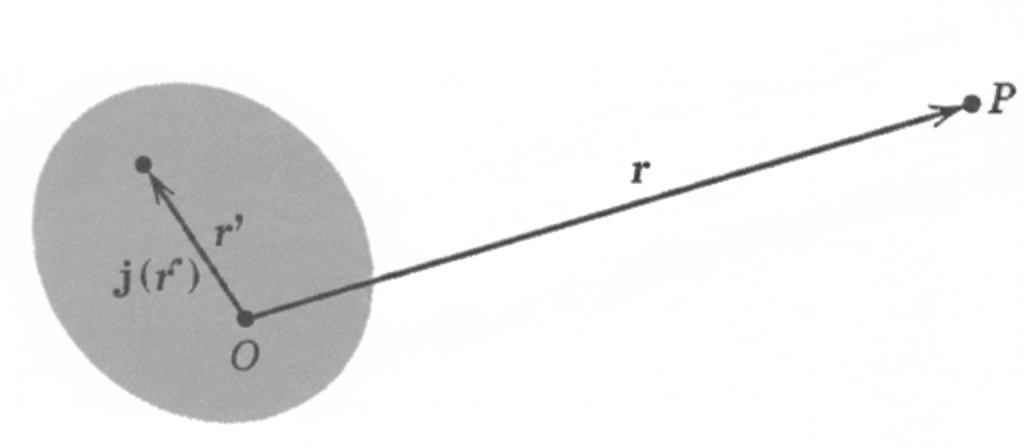
\includegraphics[width=0.5\linewidth]{figure/image49.png}
    \caption{Una distribuzione localizzata di corrente di densità $\mathbf{j} (\mathbf{r'})$ genera una distribuzione magnetica nel punto $P$ di coordinate $\mathbf{r}$}
    \label{fig:placeholder}
\end{figure}

Assumendo che $|\mathbf{r}| \gg |\mathbf{r'}|$, sviluppiamo il denominatore della \ref{eq:forma_esplicita_potenziale_vet} in serie di potenze di $\mathbf{r'}$:

\begin{equation}
    \frac{1}{|\mathbf{r} - \mathbf{r'}|} = \frac{1}{|\mathbf{r}|} + \frac{\mathbf{r} \cdot \mathbf{r'}}{|\mathbf{r}|^3} + ...
\end{equation}

Allora per ogni componente del potenziale vettore si potrà scrivere lo sviluppo

\begin{equation}
    A_i (\mathbf{r}) = \frac{\mu_0}{4 \pi} \left[ \frac{1}{|\mathbf{r}|} \int j_i (\mathbf{r'}) d^3 r' + \frac{\mathbf{r}}{|\mathbf{r}|^3} \cdot \int j_i (\mathbf{\mathbf{r'}} ) \mathbf{r'} d^3 r' + ... \right]
\end{equation}

Dato che stiamo considerando casi stazionari, dall'equazione di continuità \ref{eq:equazione_continuità}, si ha che $\nabla \cdot \mathbf{j} = 0$. \\

Possiamo andare a semplificare la predente forma sfruttando una relazione matematica, che però non dimostreremo.\\

Siano $f(\mathbf{r'})$ e $g(\mathbf{r'})$ due funzioni regolari di $\mathbf{r'}$, che specificheremo in seguito. Allora, essendo $\mathbf{j}(\mathbf{r'})$ localizzata e con divergenza nulla, vale la relazione

\begin{tcolorbox}[colback=yellow!10!white, colframe=orange!70!black, boxrule=0.8pt]
\begin{equation} \label{eq:relazione_dip_magn}
    \int (f \mathbf{j} \cdot \nabla' g + g \mathbf{j} \cdot \nabla ' f  + fg \nabla' \cdot \mathbf{j}) d^3 r' = 0
\end{equation}
\end{tcolorbox}

Ponendo $f = 1$, $g = x_i'$, dalla \ref{eq:relazione_dip_magn} con $\nabla' \cdot \mathbf{j} = 0$ si ricava 

\begin{equation*}
    \int j_i (\mathbf{r'}) d^3 r' = 0
\end{equation*}

Quindi \emph{il primo termine nello sviluppo è nullo}. \\

Ponendo $f = r_i'$ e $g = r_j '$, si ricava 

\begin{equation*}
    \int (r_i' j_j + r_j' j_i) d^3 r' = 0
\end{equation*}

Cioè 

\begin{equation*}
    \int r'_j j _i d^3 r' = - \int r'_i j_j d^3 r' 
\end{equation*}

Usando questa relazione si nota facilemnte che vale 

\begin{equation*}
    \int r_j' j_i d^3 r' = \frac{1}{2} \int (r_j' j_i- r_i' j_j) d^3 r' 
\end{equation*}

Riconoscendo il prodotto vettoriale 

\begin{equation*}
    r_j' j_i- r_i' j_j = \varepsilon_{ijk} (\mathbf{r'} \times \mathbf{j})_k
\end{equation*}

Quindi 

\begin{equation*}
    \int r_j' j_i d^3 r' = \frac{1}{2} \int \varepsilon_{ijk} (\mathbf{r'} \times \mathbf{j})_k d^3 r'
\end{equation*}

Allora l'integrale al secondo termine dell'espansione può essere trasformato 

\begin{align}
\mathbf{r} \cdot \int \mathbf{r'} \, j_i(\mathbf{r'}) \, d^3 r'
&= \sum_j r_j \int r'_j \, j_i(\mathbf{r'}) \, d^3 r' \\[6pt] \label{eq: integrale_momento_magnetico}
&= -\frac{1}{2} \sum_j r_j \int \left( r'_i j_j(\mathbf{r'}) - r'_j j_i(\mathbf{r'}) \right) d^3 r' \\[6pt]
&= -\frac{1}{2} \sum_{j,k} \varepsilon_{ijk} \, r_j \int \left( \mathbf{r'} \times \mathbf{j}(\mathbf{r'}) \right)_k \, d^3 r' \\[6pt]
&= -\frac{1}{2} \left[ \mathbf{r} \times \int \left( \mathbf{r'} \times \mathbf{j}(\mathbf{r'}) \right) d^3 r' \right]_i
\end{align}

Allora se vado a definite il \emph{momento magnetico} come \mkeyword{momento magnetico}

\begin{tcolorbox}[colback=yellow!10!white, colframe=orange!70!black, boxrule=0.8pt]
\begin{equation} \label{eq:momento_magnetico}
    \mathbf{m} = \frac{1}{2} \int\mathbf{r'} \times \mathbf{j}(\mathbf{r'}) d^3 r' 
\end{equation}
\end{tcolorbox}

Se andiamo a sostituire i risultati trovati nell'espansione, troncandola al secondo ordine si ottiene 

\begin{equation}
    \mathbf{A} (\mathbf{r}) = \frac{\mu_0}{4 \pi} \frac{\mathbf{m \times \mathbf{r}}}{|\mathbf{r}|^3}
\end{equation}

Questo è il termine non nullo di ordine più basso nello sviluppo di $\mathbf{A}$ per una distribuzione stazionaria di correnti localizzate. L'induzione magnetica $\mathbf{B}$ può essere calcolata a partire dalla definizione di potenziale vettoriale.

\begin{tcolorbox}[colback=yellow!10!white, colframe=orange!70!black, boxrule=0.8pt]
\begin{equation} \label{eq:campo_magnetico_dipolo}
    \mathbf{B = }\frac{\mu_0}{4 \pi r^3} \left[ 3 (\mathbf{m} \cdot \mathbf{u}_r) \mathbf{u}_r - \mathbf{m} \right]
\end{equation}
\end{tcolorbox}

Si nota, così, la somiglianza nella forma tra la \ref{eq:campo_magnetico_dipolo} e la \ref{eq:campo_dipolo}. \\

\section{Momento magnetico di una spira filiforme piana}

Se la corrente è costituita da una spira filiforme piana ma di forma arbitraria, il momento magnetico può essere espresso in modo molto semplice. Se $ d\mathbf{s}$ è l'elemento di linea del circuito $C$ percorso dalla corrente $i$, la \ref{eq:momento_magnetico} diventa 

\begin{equation}
    \mathbf{m} = \frac{i}{2} \oint_{C} \mathbf{r'} \times d \mathbf{s}
\end{equation}

Per una spira piana il momento magnetico è dunque perpendicolare al piano della spira. Poiché $|\mathbf{r'} \times d \mathbf{s}|/2 = d\Sigma$, dove $d \Sigma$ è l'area del triangolo elementare definito dai due estremi di $d \mathbf{s}$ e dall'origine, l'integrale di linea da l'area totale della spira. Perciò il momento magnetico può essere espresso come 

\begin{tcolorbox}[colback=yellow!10!white, colframe=orange!70!black, boxrule=0.8pt]
\begin{equation} 
    \mathbf{m} = i \Sigma \ \mathbf{u}_n
\end{equation}
\end{tcolorbox}

Dove $i$ è la corrente che scorre attraverso la spira, $\Sigma$ è l'area racchiusa dal filo e $\mathbf{u}_n$ è il versore ortogonale al piano su cui giace la spira e il cui verso si ottiene grazie alla regola della mano destra in base al verso in cui scorre la corrente.\\

\section{Dipolo magnetico elementare} 

Il risultato ottenuto mostra che, a grandi distanze, il potenziale vettore generato da una distribuzione stazionaria di correnti localizzate ha la forma

\begin{tcolorbox}[colback=yellow!10!white, colframe=orange!70!black, boxrule=0.8pt]
\begin{equation}
    \mathbf{A}(\mathbf{r}) = \frac{\mu_0}{4 \pi} \frac{\mathbf{m} \times \mathbf{r}}{r^3}
\end{equation}
\end{tcolorbox}

che dipende unicamente dal momento magnetico $\mathbf{m}$ della distribuzione.

Questo suggerisce di interpretare $\mathbf{m}$ come la quantità che caratterizza il comportamento del sistema a grandi distanze, in completa analogia con il momento di dipolo elettrico nel caso elettrostatico.\\

Si introduce quindi il concetto di \emph{dipolo magnetico} \mkeyword{dipolo magnetico} come un sistema fisico il cui campo magnetico, a grandi distanze, è descritto dalla \ref{eq:campo_magnetico_dipolo}.\\

\newpage

Il modello più semplice di dipolo magnetico è costituito da una spira circolare percorsa da corrente, sufficientemente piccola rispetto alle distanze di osservazione.

\begin{figure} [h]
    \centering
    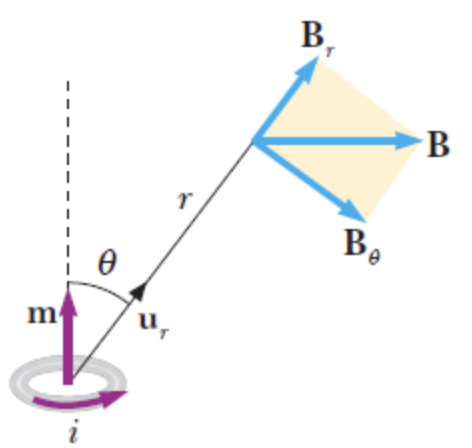
\includegraphics[width=0.5\linewidth]{figure/image50.png}
    \caption{Campo magnetico prodotto da un dipolo magnetico}
    \label{fig:placeholder}
\end{figure}

\section{Energia di un dipolo magnetico}

In analogia con quanto fatto con il dipolo elettrico, anche per il dipolo magnetico, spira o ago magnetico, si definisce un'energia potenziale, legata alla posizione angolare rispetto alla direzione di $\mathbf{B}$. \\

Consideriamo un dipolo magnetico immerso in un campo magnetico $\mathbf{B}$, la sua energia potenziale risulta essere 

\begin{tcolorbox}[colback=yellow!10!white, colframe=orange!70!black, boxrule=0.8pt]
\begin{equation}
    U_p = - \mathbf{m} \cdot \mathbf{B} = - mB \cos \theta = - i \Sigma B \cos \theta
\end{equation}
\end{tcolorbox}

A partire da questa definizione, allora, è possibile trovare anche un'espressione per la forza $\mathbf{F}$ che agisce sul dipolo. 

\begin{tcolorbox}[colback=yellow!10!white, colframe=orange!70!black, boxrule=0.8pt]
\begin{equation}
    \mathbf{F} = - \nabla U_p = \nabla (\mathbf{m} \cdot \mathbf{B})
\end{equation}
\end{tcolorbox}

\section{Momento meccanico di un dipolo magnetico}

In analogia con quanto fatto con il dipolo elettrico, anche per il dipolo magnetico, spira o ago magnetico, si definisce un momento meccanico, legato alla posizione angolare rispetto alla direzione di $\mathbf{B}$. \\

Consideriamo un dipolo magnetico immerso in un campo magnetico $\mathbf{B}$, il momento meccanico che agisce sul dipolo risulta essere 

\begin{tcolorbox}[colback=yellow!10!white, colframe=orange!70!black, boxrule=0.8pt]
\begin{equation}
    \mathbf{M} = \mathbf{m} \times \mathbf{B} = - m B \sin \theta \ \mathbf{u}_z = - \frac{\partial U_p}{\partial \theta} \ \mathbf{u}_z
\end{equation}
\end{tcolorbox}

\subsection{Interazione tra dipoli}

\section{Espressioni di forza, momento e lavoro tramite il flusso magnetico}

Consideriamo un circuito qualsiasi $C$, anche non piano, percorso dalla corrente $i$ e una qualsiasi superficie $\Sigma$ che abbia il circuito $C$ come contorno. Il circuito è immerso in un campo magnetico $\mathbf{B}$, anche non uniforme. \\

Estendiamo alla superficie $\Sigma$ l'argomento della suddivisione in tanti piccoli circuiti rettangolari, tutti percorsi dalla stessa corrente $i$ e concordemente orientati. 

\begin{figure} [h]
    \centering
    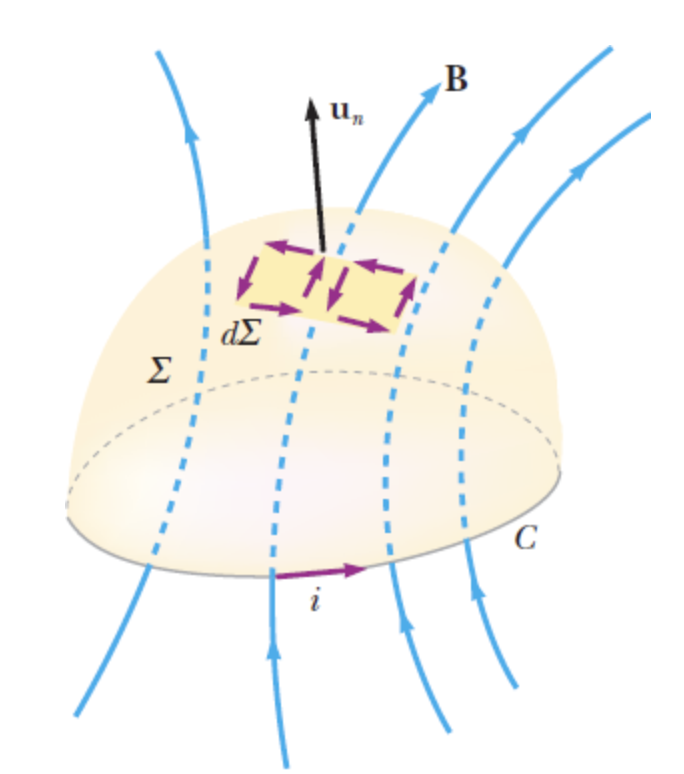
\includegraphics[width=0.5\linewidth]{figure/image51.png}
    \caption{}
    \label{fig:placeholder}
\end{figure}

L'energia potenziale del generico circuito di area $d\Sigma$ è 

\begin{equation*}
    d U_p = - d \mathbf{m} \cdot \mathbf{B} = - i \mathbf{B} \cdot \mathbf{u}_n \ d \Sigma = -i \ d\Phi (\mathbf{B})
\end{equation*}

dove $d \Phi (\mathbf{B})$ è il flusso infinitesimale di $\mathbf{B}$ attraverso $d \Sigma$. Integrando sulla superficie $\Sigma$ si ottiene l'energia potenziale del circuito $C$

\begin{tcolorbox}[colback=yellow!10!white, colframe=orange!70!black, boxrule=0.8pt]
\begin{equation}
    U_p = -i \int \mathbf{B} \cdot \mathbf{u}_n \ d \Sigma = -i \Phi (\mathbf{B})
\end{equation}
\end{tcolorbox}

L'energia potenziale di un circuito percorso da corrente $i$ e immerso in un campo magnetico $\mathbf{B}$ è eguale all'opposto del prodotto della corrente $i$ per il flusso di $\mathbf{B}$ concatenato col circuito.\\

Dato che $\mathbf{B}$ è solinoidale, il suo flusso non dipende dalla particolare $\Sigma$ che ha il circuito come contorno, ma solo dal contorno. 

A seguito di uno spostamento rigido o di una deformazione il flusso magnetico attraverso il circuito può cambiare e indichiamo con $d \Phi$ la variazione infinitesima di flusso. 
Nel processo viene compiuto, dalle forze del campo, il lavoro elementare

\begin{equation}
    dW = - dU_p = i \ d \Phi (\mathbf{B})
\end{equation}

Per una variazione finita da una configurazione iniziale 1 a una finale 2 il lavoro complessivo vale 

\begin{tcolorbox}[colback=yellow!10!white, colframe=orange!70!black, boxrule=0.8pt]
\begin{equation}
    W = i \Delta \Phi (\mathbf{B}) = i (\Phi_2 (\mathbf{B}) - \Phi_1 (\mathbf{B}))
\end{equation}
\end{tcolorbox}

\'E essenziale, per la validità delle formule trovate, che durante il processo la corrente resti costante.\\

Dalla relazione sopra, allora si ottiene che per una generica spira immersa in un campo magnetico vale 

\begin{tcolorbox}[colback=yellow!10!white, colframe=orange!70!black, boxrule=0.8pt]
\begin{equation}
    \mathbf{F} = i \nabla \Phi (\mathbf{B})
\end{equation}
\end{tcolorbox}

Mentre per il momento meccanico

\begin{tcolorbox}[colback=yellow!10!white, colframe=orange!70!black, boxrule=0.8pt]
\begin{equation}
    M = i \frac{\partial \Phi (\mathbf{B})}{\partial \theta} = - \frac{\partial U_p}{\partial \theta}
\end{equation}
\end{tcolorbox}
